
\section{Notes}

% Hornkjøl et al \cite{hornkjol2022csf} report of peak CSF flow
% velocites in the SAS of 20, 40 and 50 \mu m/s, with lower values < 4
% \mu m/s along the upper convexity for
% non-parasagittal-dura-efflux-models. How do ours compare?

%% Takizawa et al \cite{takizawa2017characterization} report of cardiac and respiratory-driven CSF velocity magnitudes of $\approx$ 0.21 cm/s and 0.11 cm/s, respectively, in the aqueduct and $\approx$ 1.0 cm/s and 0.33 cm/s at the foramen magnum. These values are compatible, though somewhat lower, than our peak flow speeds of 19.8 cm/s for the cardiac contribution and 4.8 cm/s for the respiratory. Similarly, Yildiz et al \cite{yildiz2017quantifying} report of peak CSF velocities associated with cardiac and respiratory pulsatility on the order of 0.97 $\pm$ 0.33 cm/s and 0.58 $\pm$ 0.40 cm/s at the foramen magnum. Vinje et al \cite{vinje2019respiratory} simulate CSF flows in the aqueduct with peak velocities ranging from $\approx$ 2 cm/s to 10 cm/s depending on the aqueduct geometry. Our cross-section CSF velocities at the foramen magnum reduce to 7.7 cm/s for the cardiac and 1.4 cm/s for the respiratory (Slack communication, Jan 14, MER/MC). 

% MER: This seems to be a poster. Omitted for now. \cite{ayansiji2025p174}.}

Various notes associated with \cite{eide2024functional}:
\begin{itemize}
  \item
    Can observations of tracer indicate compartmentalization without
    the existence of physical barriers but in the presence of
    e.g.~substantial flow? We made observations in this direction in
    \cite{vinje2021brain}, relating to the then-active
    shape-of-perivascular-spaces discussion. We can address this by
    trying to quantify and evaluate the permeability of the PVS-SAS
    interface - comparing model predictions with the timings and
    patterns presented by \cite{eide2024functional}.
  \item
    Do the tracer primarily move from the PVS into the SAS or along
    (more slowly) along the SAS? This is left as an open question by
    \cite{eide2024functional} (page 3)
  \item
    How do altered ICP affect transport? Note that PVSAS transport is
    impaired (delayed) with increasing mean wave amplitude in the ICP
    signal and for iNPH patients (with enlarged PVSAS spaces).
  \item
    Very useful reference for PVS sizes (10--20 mm$^2$ in reference
    patients, 15-70 mm$^2$ in iNPH), and average propagation speeds.
\end{itemize}

%% We investigate the PVS flow velocities resulting from a transmantle pressure gradient, cardiac peristalsis and vasomotion-induced flow in a reconstructed arterial network and illustrate the effect of the obtained PVS flow fields on the spreading patterns of intrathecally injected tracer. Further, we explore whether solutes move exclusively from the PVS to the SAS, or bidirectionally along both pathways by comparison of first-time arrival times along major cerebral arteries.

%\paragraph{PVS Flow velocities}
%% To investigate PVS flow velocities, we extract the centerlines and associated radii of the arterial network from data \cite{hodneland2019new}, and label the main cerebral arteries (Figure 3A+C). We consider three different PVS flow fields: flow driven by CSF production-induced pressure differences, cardiac peristaltic flow, and vasomotion peristaltic flow (\Cref{fig:pvs}B). Pressure-driven flow velocities are computed by solving one-dimensional flow equations with pressure boundary conditions derived from the production field. Cardiac- and vasomotion-driven PVS flow velocities are obtained from semi-analytical estimates for peristaltic flow, assuming a frequency of 1\,Hz, a 1\,\% radius change, and a wavelength of 2 meters for cardiac flow, and a frequency of 0.1\,Hz, a 10\,\% radius change, and a wavelength of 2\,cm for vasomotion.

%% The production-driven pressure gradient induces low flow velocities, with an average velocity of 0.08\,\textmu m and a maximum velocity of 0.55\,\textmu m (\Cref{fig:csf}D+H). In contrast, cardiac-driven velocities are approximately one order of magnitude higher, with an average velocity of 0.92\,\textmu m and a maximum velocity of 7.31\,\textmu m (\Cref{fig:pvs}E+H). Vasomotion-driven PVS flow reach substantially higher velocities, up to 54\,\textmu m, with an average of 13.05\,\textmu m. For all drivers of PVS flow, the majority of flow occurred in the direction of blood flow, with only a small fraction in the opposing direction (\Cref{fig:pvs}H).

%\paragraph{Differences in PVS flow velocities substantially alter tracer enrichment patterns around major cerebral arteries}

%% Using the computed PVS flow velocities, we predict the effect of rapid PVS flow on intracranial transport by comparing a slow transport model (pressure-driven and cardiac-driven PVS flow) with a high-velocity model that accounts for all three mechanisms (pressure-, cardiac-, and vasomotion-driven). In both models, tracers were first observed 48 minutes after injection at the basal artery (\Cref{fig:pvs}G), defined by the first-time arrival (FTA), the time at which concentration first exceeds $0.1\,$mmol/l.

%% At all upstream locations along the middle cerebral arteries (MCAs) and anterior cerebral artery (ACA), we found substantially reduced FTAs in the rapid PVS flow model (\Cref{fig:pvs}G+N). Furthermore, peak concentrations in the PVS were attained earlier than in the surrounding tissue (0:48h / 1:12h at the MCA and 1:00h / 1:48h at MCA2) in the vasomotion model, while concentrations peaked more simultaneously in the low-velocity model. The earlier occurrence and delay in peak time between the PVS and surrounding tissue indicate the directionality of tracer enrichment — it first arrives in the PVS and subsequently spreads into the tissue and SAS, especially in the vasomotion model.

%% The difference in tracer spreading observed at the MCA/ACA points also holds on an aggregated level in the whole arterial PVS. Computing the total amount of tracer in the PVS depending on the distance to the arterial network's inlet nodes (basal artery (BA), left internal carotid artery (ICA-L), or right internal carotid artery (ICA-R)), we find more rapid transport of tracer in the vasomotion model. We also investigate the potential effect of increased dispersion in the PVS, finding that adding a dispersion enhancement factor of 100 in the PVS only induced minor changes in the global spreading rate (\Cref{fig:pvs}J). However, differences in tracer transport along the PVS translate to altered enrichment patterns on a whole-organ scale. For instance, after 4-6 hours, the faster-moving tracer in the PVS is clearly visible in the adjacent spaces of the ACA, MCA, and other arteries in sagittal, coronal, and axial planes of the whole organ (\Cref{fig:pvs}O). In contrast, the model with only pressure- and cardiac-driven PVS flow does not exhibit clear signs of accelerated tracer transport along the PVS.

%Flow of CSF through the SAS and the ventricular system is a crucial driver of transport in the human brain environment.
%While cardiac- and respiratory induced oscillatory flow increases mixing, the production of CSF in the choroid plexus creates a steady advective flow within the CSF-filled spaces of the cranium \cite{hornkjol2022csf}. 
%We construct a 3D model of the SAS and the ventricular system (\Cref{fig:csf}A,B and C) and compute CSF flow fields for three different scenarios: CSF production in the choroid plexus, CSF flow at systolic peak blood inflow and CSF flow in response to free breathing.

% production flow simulation
%% To simulate the production-driven flow, we impose an inflow of $400\,$ml/day across the surface of the lateral ventricle and allow a resistive outflow across the upper convexity of the arachnoid mater, leading to a total pressure drop of $26\,$mPa between the production and outflow sites (\Cref{fig:csf}D). A maximum flow velocity of $1.8\,$mm/s is attained in the aqueduct, while the mean velocity in the SAS is $2.6\,\mu$m/s (\Cref{fig:csf} E).


%% % cardiac pulsatility
%% Assessing the effect of cardiac-driven dispersion, we compute a steady CSF flow field at peak systolic blood inflow. We mimic the resulting reduction of CSF space volume by imposing an inflow of $6\,$ml/s \cite{baledent2014imaging, causemann2022human} and $0.31\,$ml/s \cite{vinje2019respiratory} across the upper arachnoid mater ($\Gamma_{\rm AM-U}$) and the lateral ventricle ($\Gamma_{\rm VL}$) surface, respectively. We allow free outflow into the spinal SAS ($\Gamma_{\rm SSAS}$). In addition, we upscale the obtained pressure field to account for the lack of pulsatile inertial effects in our model (see \Cref{sec:csf_dispersion}). In this scenario, we observe a pressure drop of $10\,$Pa between lateral ventricles and the spinal SAS and a maximum flow velocity of $19.8\,$cm/s in the aqueduct (\Cref{fig:csf}F and J).
%% Next, we estimate a spatially varying dispersion enhancement factor $R$ from cardiac-induced pulsatility by combining the computed pressure field with the theory of shear-augmented dispersion (see \Cref{sec:csf_dispersion}). Assuming a cardiac frequency of $1\,$Hz, we find that cardiac-induced pulsatile CSF flow increases the effective diffusion by more than two orders of magnitude in the aqueduct and around the cisterna magna, but has little effect in most of the SAS ($R < 1$) (\Cref{fig:csf} G and K). 

%% % respiratory pulsatility
%% Employing the same methodology, we estimate the respiratory contribution to dispersive mixing by computing the CSF flow field driven by an inflow of $0.121\,$ml/s \cite{liu2024using} and $1\,$ml/s \cite{gutierrez2022effect} across the lateral ventricular wall and the arachnoid mater, respectively. This amounts to a respiratory peak flow volume of $1.121\,$ ml/s at the craniocervical junction. While the resulting flow velocities are only about one fourth of their cardiac-induced counterparts (see \Cref{fig:csf}H and L), respiratory dispersive mixing reaches a factor of up to 350 due the lower respiratory frequency of $0.25\,$Hz (\Cref{fig:csf}I and M).


%% % tracer trajectory of the standard model
%% \mer{MER: I moved this to Results 1 and condensed it a little bit}
%% \mar{Next, we use the computed advective velocity field and dispersion enhancement factors to predict the spreading of $0.5\,$mmol intrathecally injected Gadobutrol in CSF-filled spaces, the parenchymal tissue and PVSs around arteries and veines. We assume pressure-driven flow in arterial and venous PVSs, and cardiac peristaltic flow in the arterial network (\Cref{sec:pvs_flow_results}). One hour post-injection, tracer moves upwards in the SAS frontally of the brainstem,  and quickly reaches supratentorial regions (\Cref{fig:csf}N). Here, it spreads both posteriorly through quadrigeminal cistern and longitudinal fissure, and anteriorly through the outer SAS, reaching the top of the cerebral cortex after around 12 h. After 24h, the tracer covers most of the brains surface (with exception of some posterior regions) and has penetrated several centimeters into the parenchymal tissue.
%% This pattern of transport is reflected in the mean tracer concentrations in each compartment, where the CSF space reaches its peak of $1.4\,$mmol/l after 2 hours, followed by the the arterial PVS concentration peak ($2.9\,$mmol/l after 4 hours) (\Cref{fig:csf}P).  While the mean concentrations in these compartments fall quickly soon after their peaks, the parenchymal tissue slowly enriches with tracer over the first 24 hours, with a final value of $0.3\,$ mmol/l.
%% Overall, about 40\,\% of the total amount of tracer remains in the cranium 24\,h post-injection, with the largest share in the CSF (53\,\%), followed by the parenchyma (35\,\%), the venous PVS (8\,\%) and the arterial PVS (5\,\%). (\cref{fig:csf}O).}

 \section{Introduction}
It remains an open question however how these physical and
physiological mechanisms, though well-characterized when viewed in
isolation, contribute to enhance human intracranial molecular
transport.

PVS flow is important as shown by experimental studies. This is being
corroborated by clinical studies in humans (Eide and Ringstad (2024),
and the new one). However, a number of open questions remain: to what
extent are PVSs compartmentalized, how fast is the flow in human PVS,
what is the effect of dilated PVS as seen in disease cases etc.  Also,
open questions on transport characteristics of the CSF spaces - what
gives the individual variations in tracer enhancements? 

What is known is that fluid motion (in the ventricular system and SAS,
in perivascular spaces, and possibly within the parenchyma) and
pulsatility play key
roles. Glymphatics~\cite{iliff2012paravascular}. Diffusion, PVS flow
and dispersion, CSF flow. Molecular transport in perivascular spaces
(PVSs) is established as a key pathway for human brain clearance and
delivery. Previous studies indicate that molecules move rapidly in the
subarachnoid space (SAS) and in PVSs surrounding pial arteries. CSF
production in the choroid plexus and possibly in the parenchyma. CSF
efflux pathways, meningeal lympahtics, nerve routes. See also to
Cserr, Phys Rev., 1971, bulk convective flow may be more important for
larger species (larger distances) and larger molecules. Contribution
both from net flow (convection) and pulsatility (mixing) both in the
CSF spaces and in PVSs. Some aspects are better established, such as;
while other factors are more disputed such as ... contribution of
vasomotion. Moreover, the role of local effects in the bigger picture
has remained hard to evaluate.

\section{Results}

\mer{MER: Old, revisit to see if we have forgotten any of these interesting ideas.}
\subsection*{Effect of interfaces (interface permeability)}

\begin{itemize}
    \item Model 0 (baseline): only diffusion, different diffusion coefficient in the parenchyma and SAS/PVS. No leak to vasculature (zero permeability). $\infty$ $\zeta_0$ at the PVS-SAS interface, $\zeta_1$ at the PVS-SAS interface. Koch et al could be a reference for PVS-parenchyma, maybe Tithof et al (2022, "A network model" ...) could give some ideas for parameters, also see Mestre et al, Nature comms, 2022. 
    \item 
    With altered interface permeabilities in the PVS (Model 1), and or in the parenchyma (Model 2) 
    \end{itemize}


\subsection*{Effect of convection}
\begin{itemize}
    \item 
    With convective flow in the PVS (zero flow in the parenchyma for now)
    \begin{itemize}
        \item 
        Model 3: PVS flow equal to 18.7 $\mu$m/s
        \item 
        Model 4: Better PVS flow (distributed, according to conservation of mass, assumptions on PVS area)
    \end{itemize}    
    \item 
    With convective flow in the ECS (out of scope here, for follow-up work?)
\end{itemize}

\begin{figure}
    \centering
    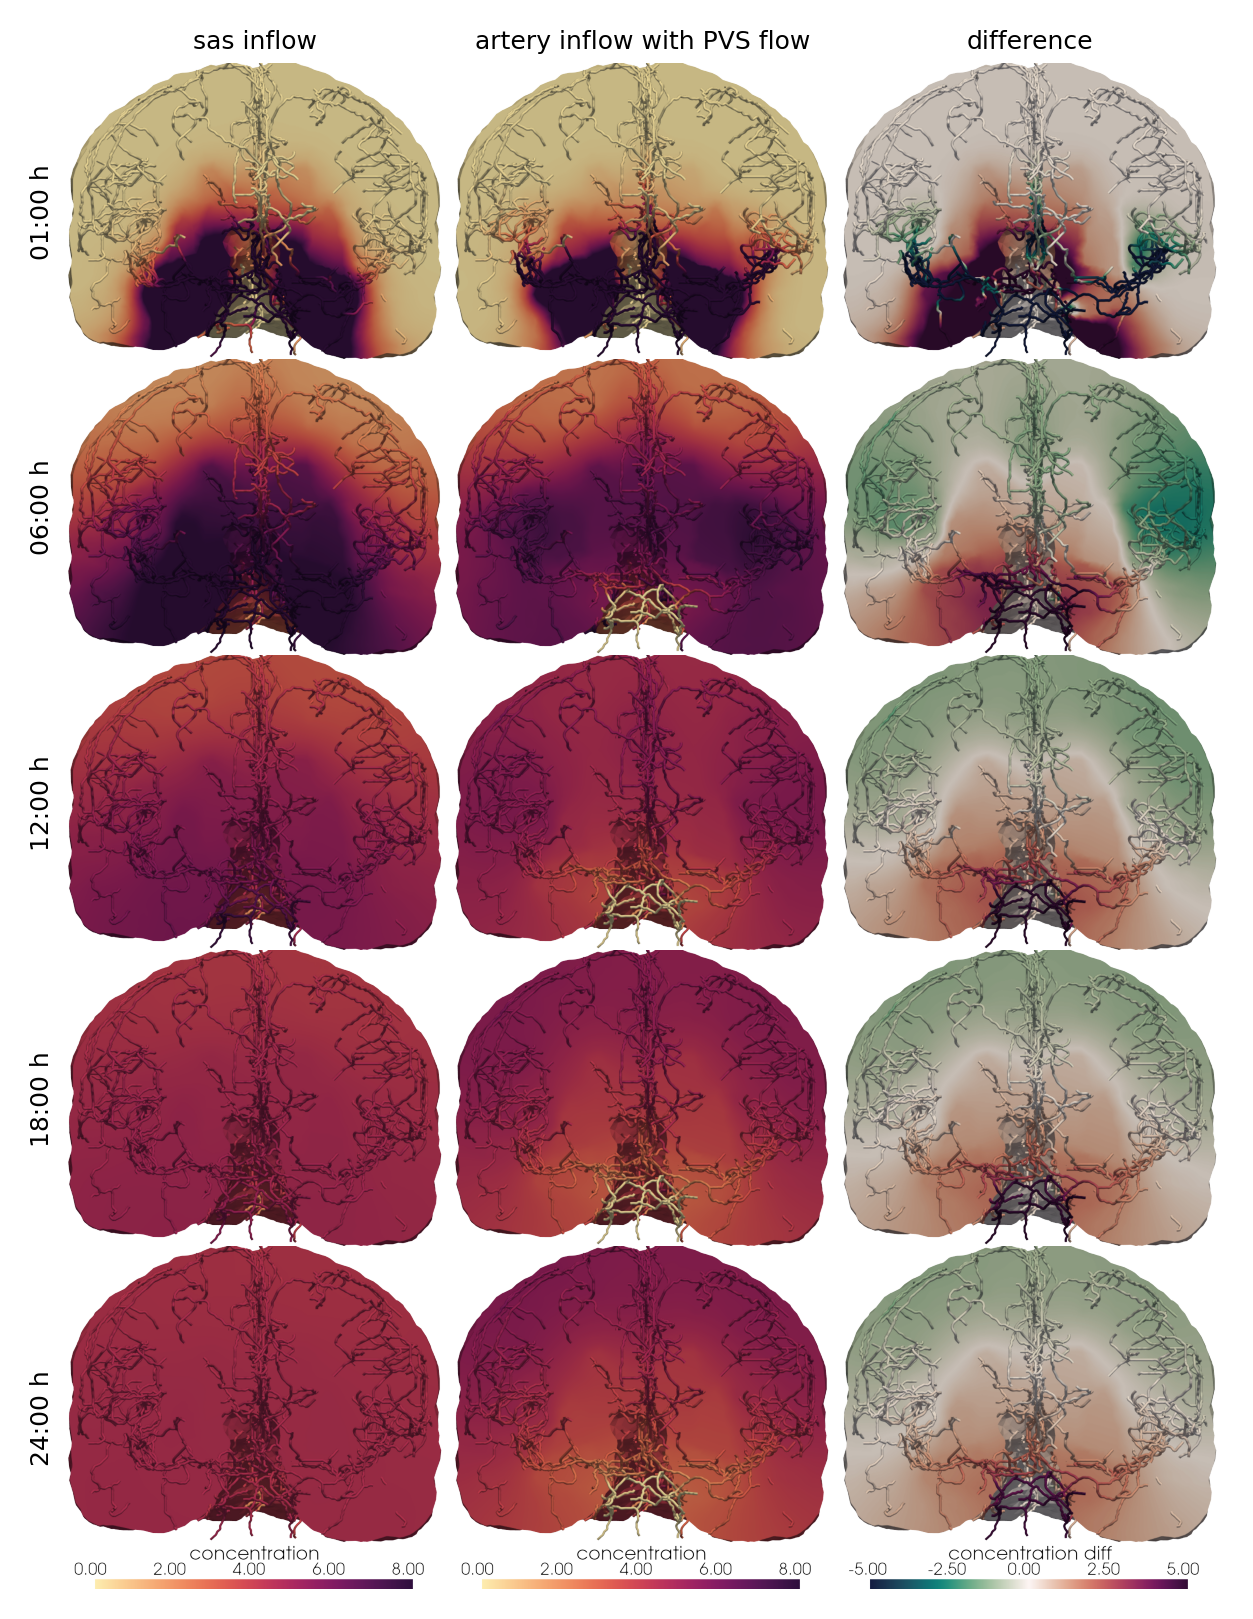
\includegraphics[width = 0.9 \textwidth]{modelB_modelC_overview.png}
    \caption{Tracer concentrations for a purely diffusive model with tracer inflow via the CSF-filled space (left) and a convective model with Tracer inflow via the arterial PVS (middle) and their difference (right) at 1, 6, 12, 18 and 24 hours after injection.}
    \label{fig:2}
\end{figure}

\subsection*{Effect of pia}
  
Effect of pia permeability (Model N-1)    

\begin{figure}
     \centering
     \begin{subfigure}[b]{0.33\textwidth}
         \centering
         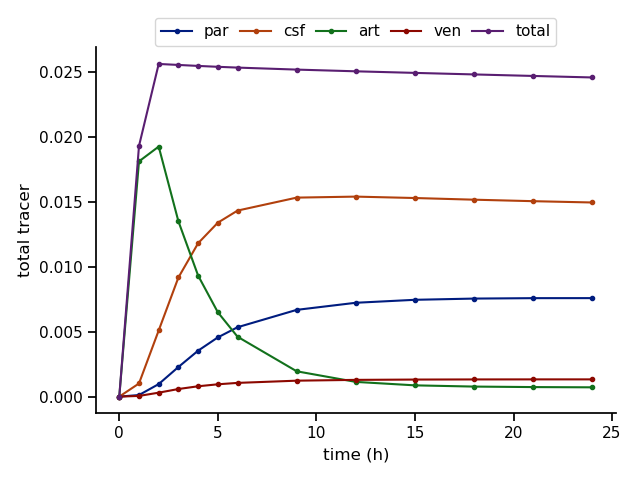
\includegraphics[width=\textwidth]{modelA_total_conc.png}
         \caption{arterial inflow, pure diffusion}
         \label{fig:y equals x}
     \end{subfigure}
     \hfill
     \begin{subfigure}[b]{0.33\textwidth}
         \centering
         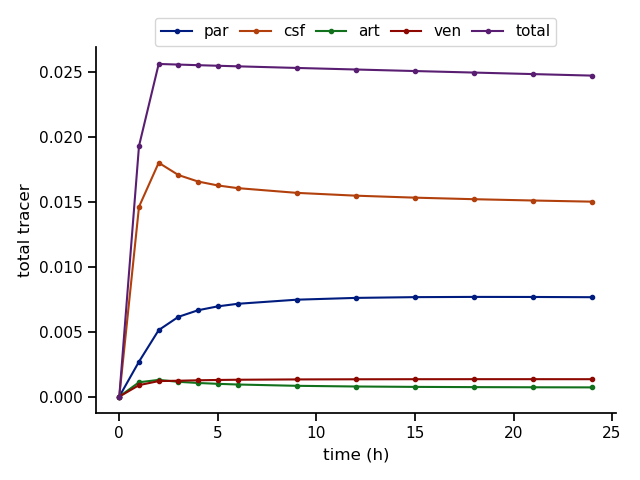
\includegraphics[width=\textwidth]{modelB_total_conc.png}
         \caption{SAS inflow, pure diffusion}
         \label{fig:three sin x}
     \end{subfigure}
     \hfill
     \begin{subfigure}[b]{0.33\textwidth}
         \centering
         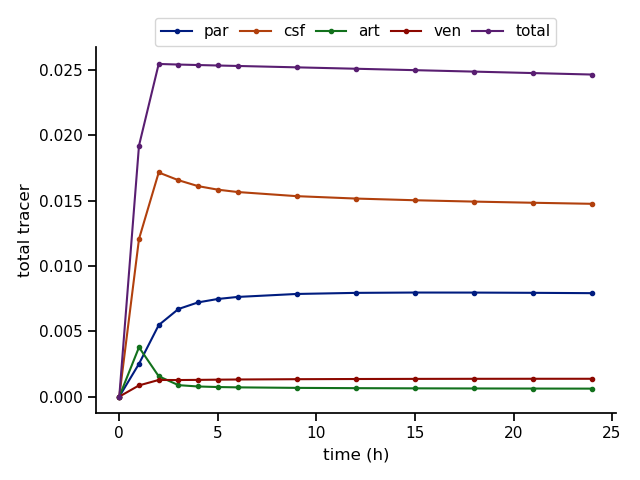
\includegraphics[width=\textwidth]{modelC_total_conc.png}
         \caption{arterial inflow, diffusion + PVS convection}
         \label{fig:five over x}
     \end{subfigure}
        \caption{Total tracer amount in parenchyma, CSF, arterial PVS and venous PVS}
        \label{fig:three graphs}
\end{figure}

\begin{figure}
\begin{subfigure}{0.5 \linewidth}
    \centering
    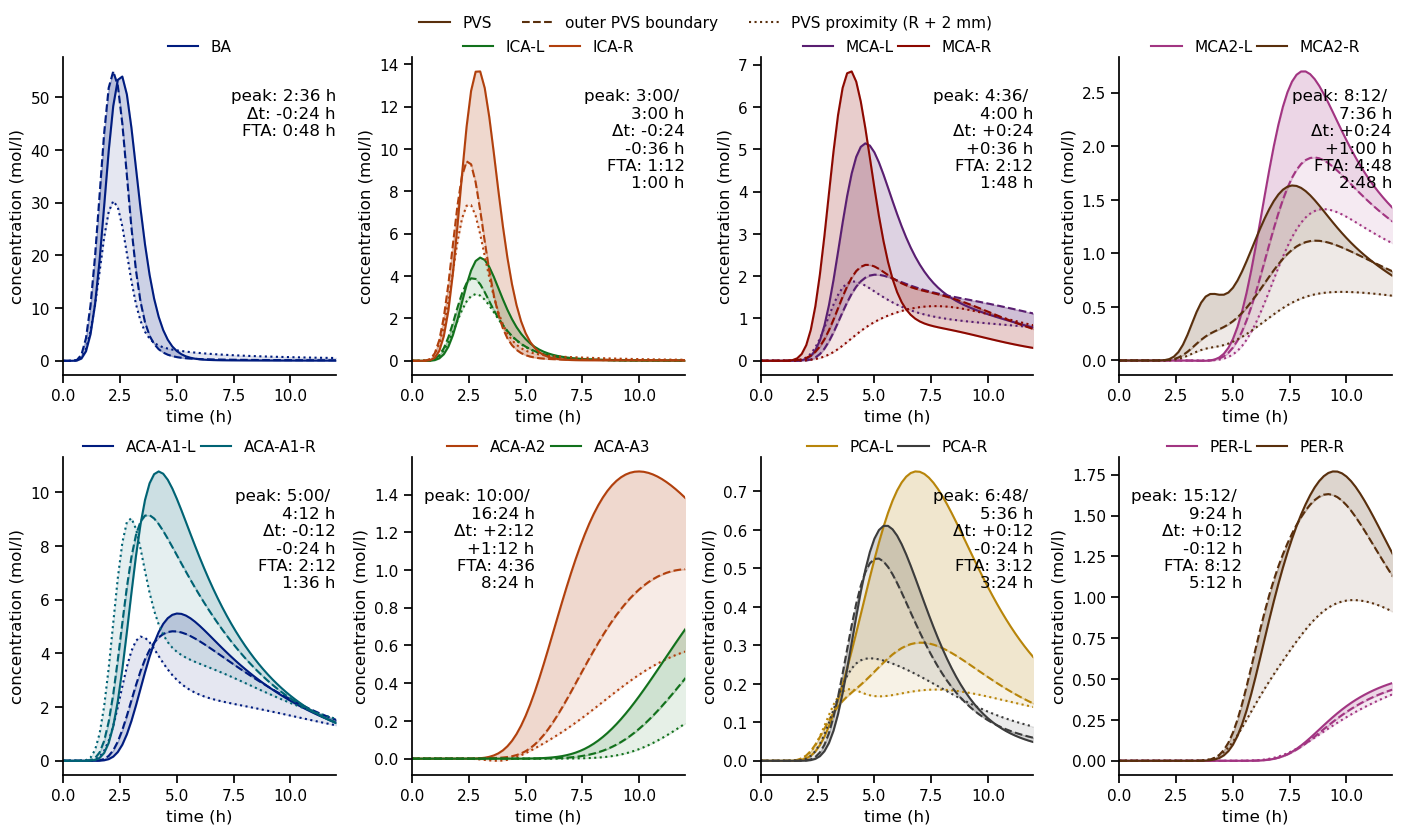
\includegraphics[width=1\linewidth]{figures/modelA_conc_at_label.png}
    \caption{B1 - $\xi$}
    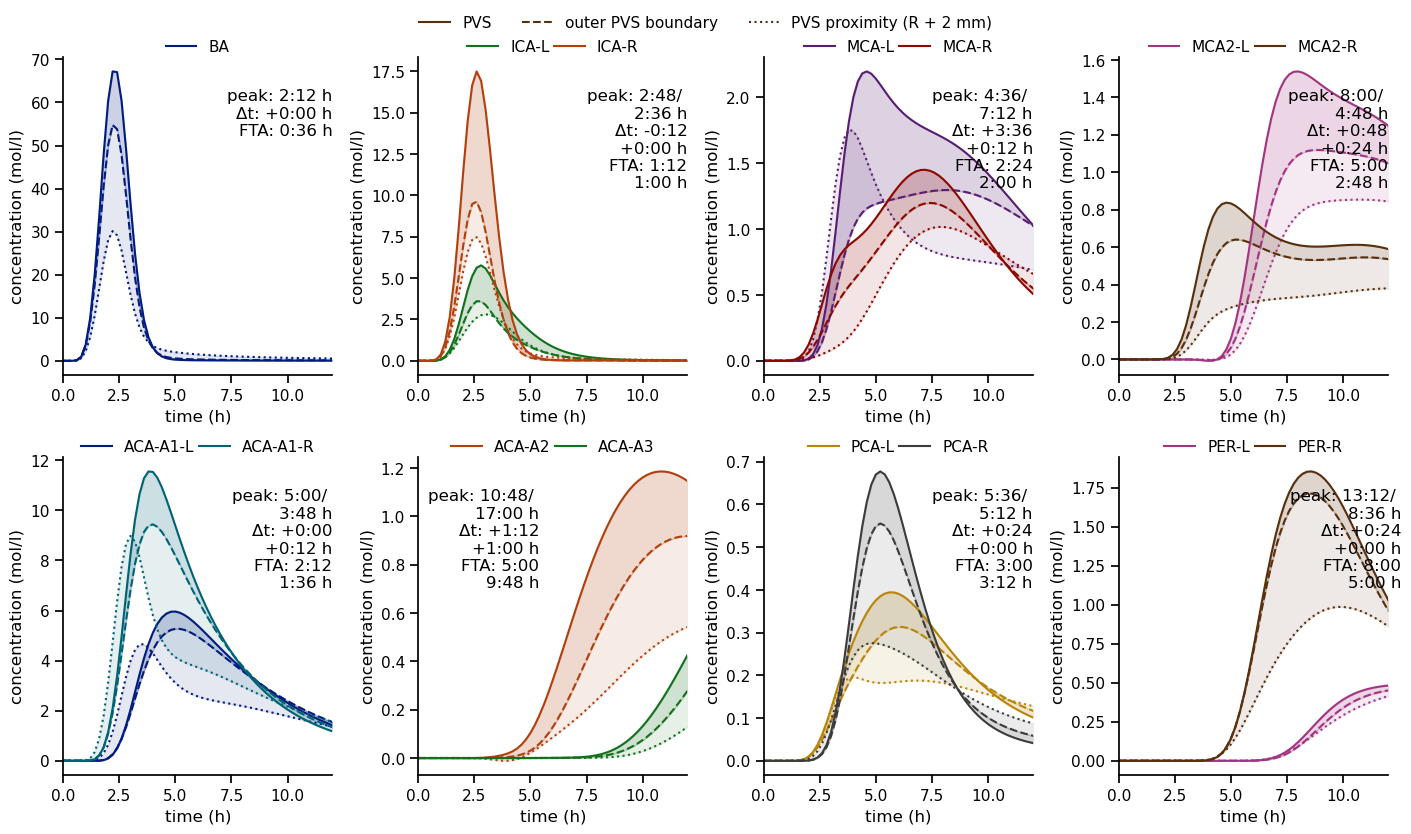
\includegraphics[width=1\linewidth]{figures/modelB1-10_conc_at_label.png}
    \caption{B1 - $10 \xi$}
    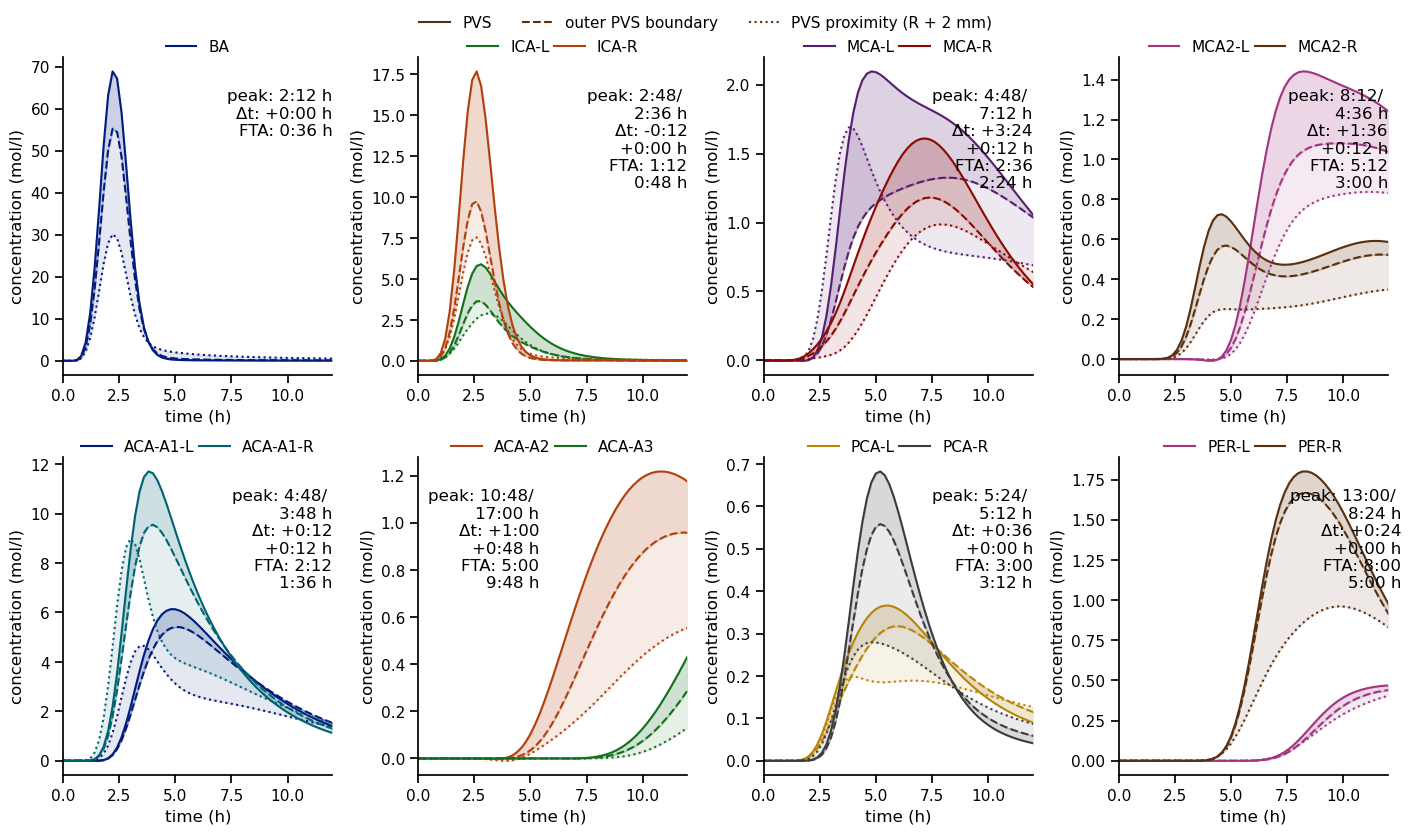
\includegraphics[width=1\linewidth]{figures/modelB1-100_conc_at_label.png}
    \caption{B1 - $100 \xi$}
    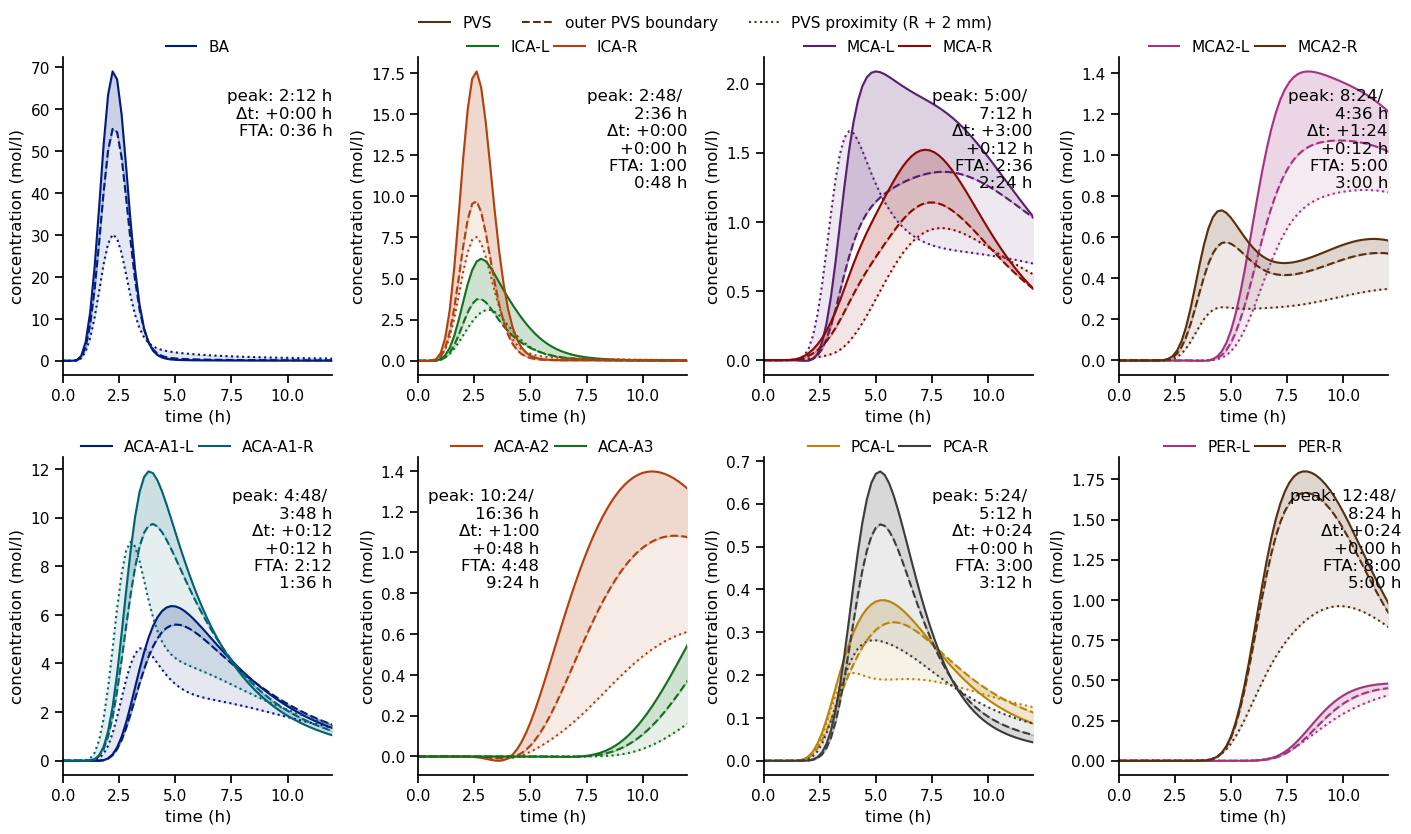
\includegraphics[width=1\linewidth]{figures/modelB1-1000_conc_at_label.png}
    \caption{B1 - $1000 \xi$}
\end{subfigure}
\begin{subfigure}{0.5 \linewidth}
    \centering
    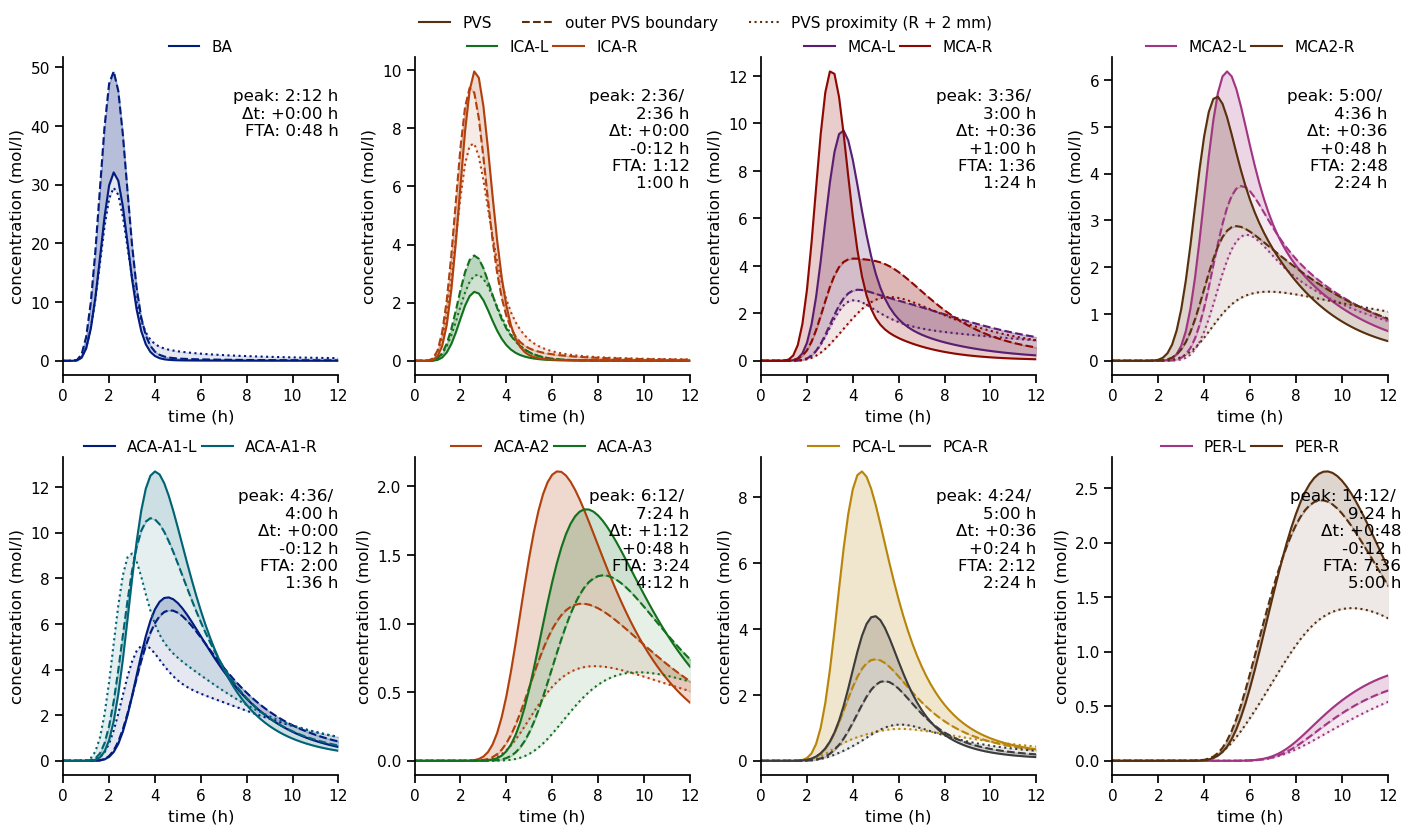
\includegraphics[width=1\linewidth]{figures/modelB2-1_conc_at_label.png}
    \caption{B2 - $\xi$}
    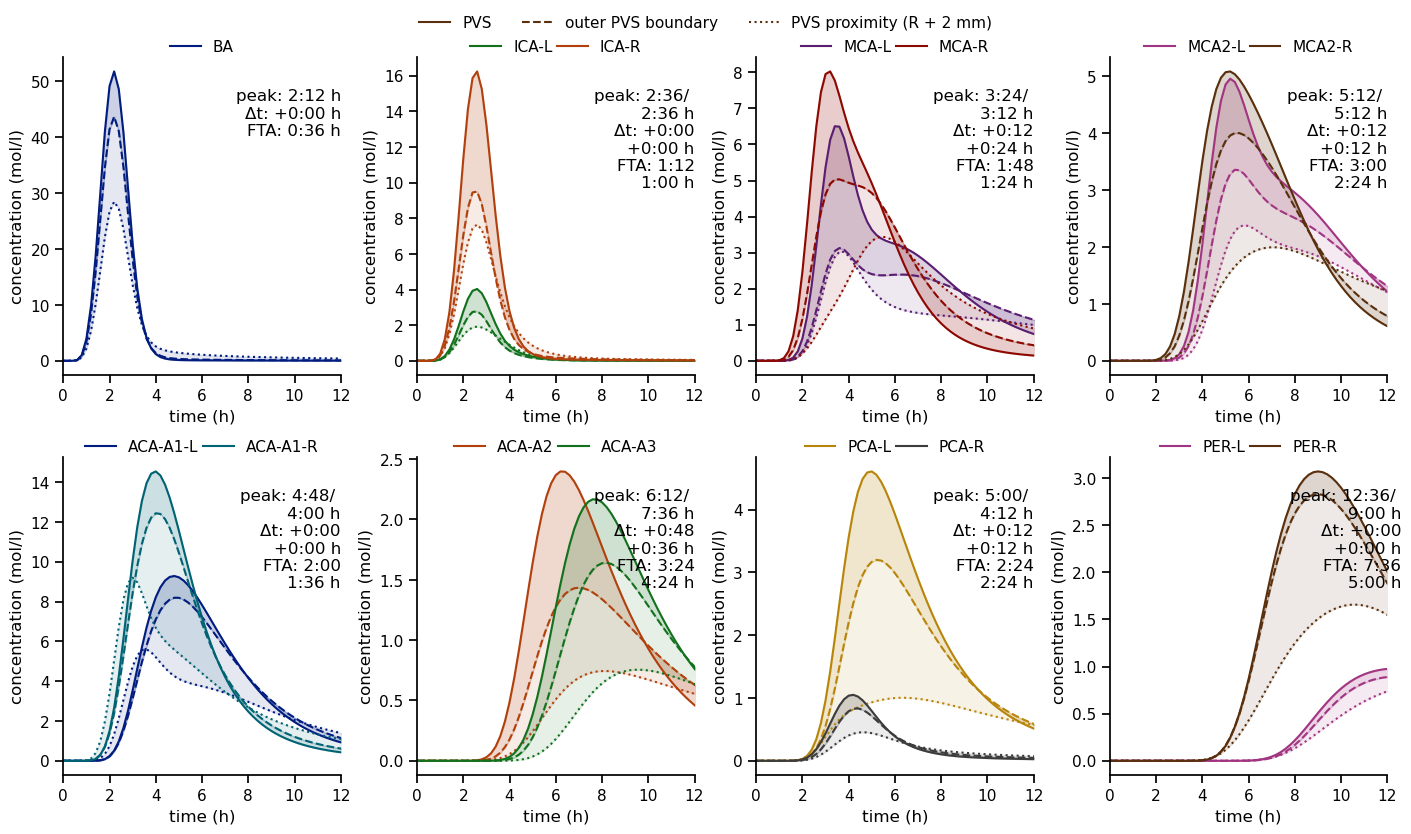
\includegraphics[width=1\linewidth]{figures/modelB2-10_conc_at_label.png}
    \caption{B2 - $10 \xi$}
    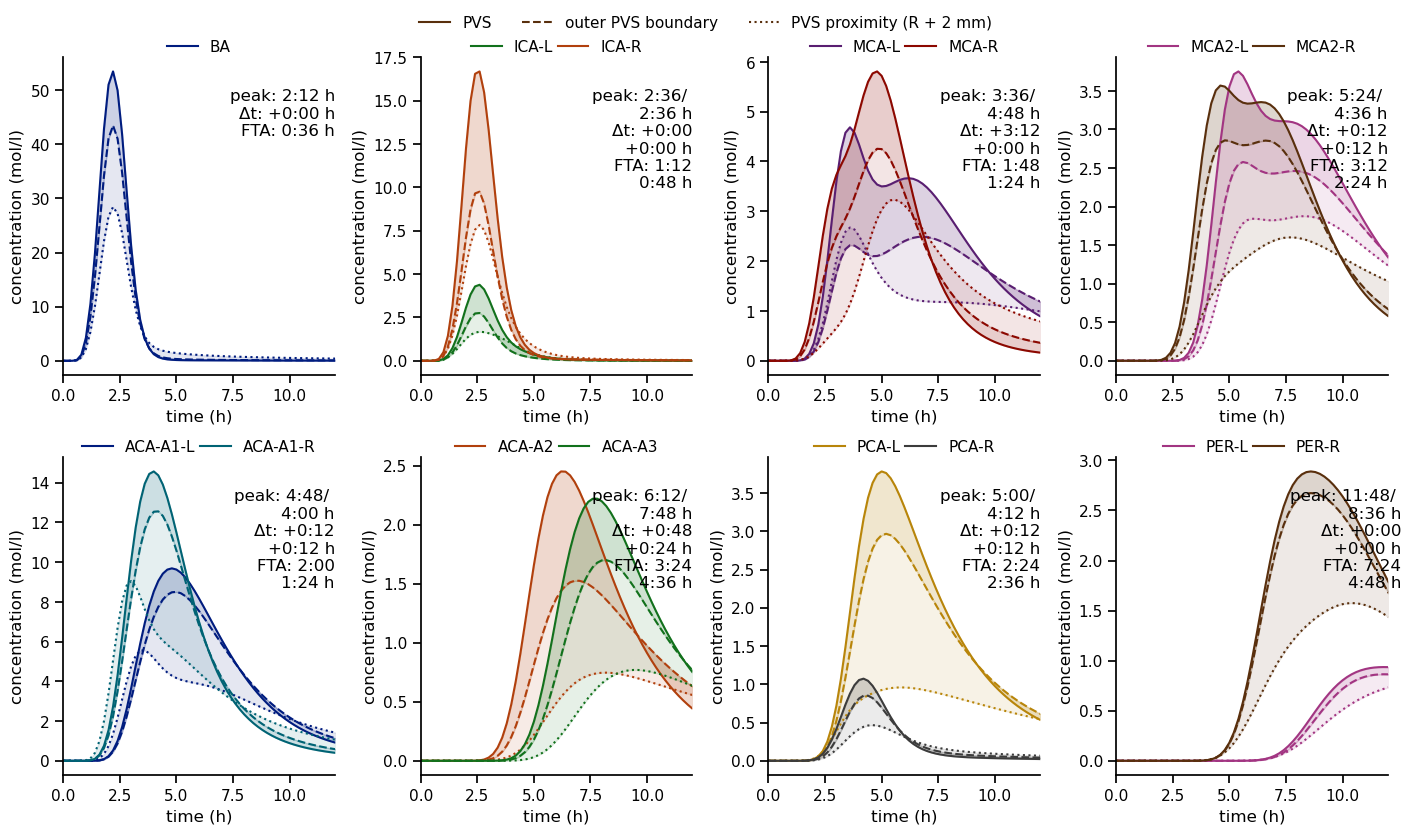
\includegraphics[width=1\linewidth]{figures/modelB2-100_conc_at_label.png}
    \caption{B2 - $100 \xi$}
    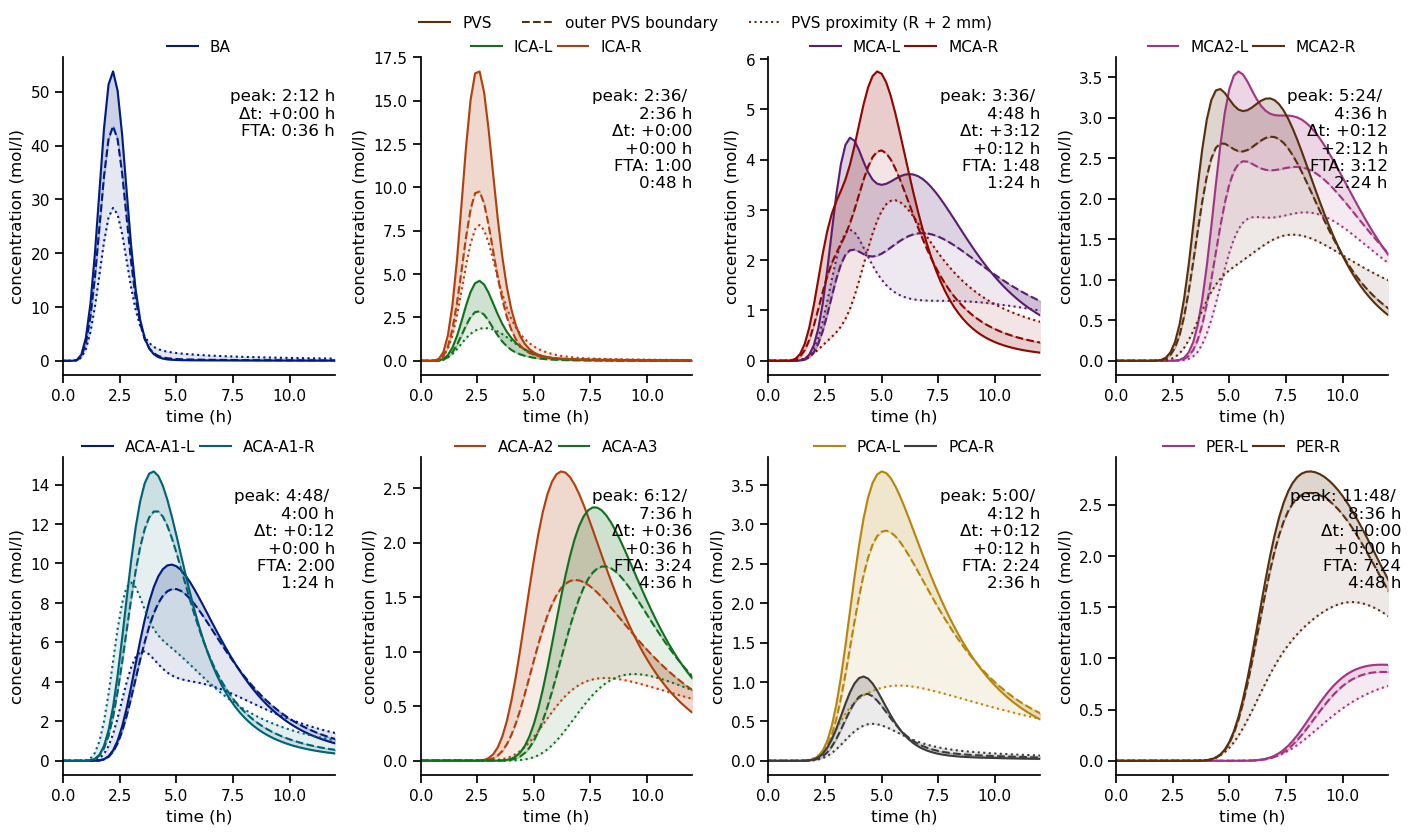
\includegraphics[width=1\linewidth]{figures/modelB2-1000_conc_at_label.png}
    \caption{B2 - $1000 \xi$}
\end{subfigure}
    \label{fig:modelB_xi_variations}
\end{figure}



\section{Foo}

We consider non-zero convection in the CSF space $u_{\rm CSF} \not = 0$ in \eqref{eq:multi_transport_3d} resulting from steady state CSF production.  Recall that $\Omega_{\mathrm{CSF}}$ represents the CSF space and that $\Gamma_{\mathrm{skull^{u/l}}}$ and $\Gamma_{\mathrm{pia}}$, $\Gamma_{\mathrm{LV}}$ represent the boundaries facing the upper and lower parts of the dura, the pia and the lateral ventricles, respectively.  Assuming CSF production in the choroid plexus located at the lateral ventricle wall, we solve the  steady state Stokes equations for the velocity and the pressure $(\bm u_{\mathrm{CSF}}, p_{\mathrm{CSF}})$ in the CSF domain: 
\begin{subequations}
    \begin{alignat}{2}
 - \mu \Delta \bm u_{\mathrm{CSF}} + \nabla p_{\rm{CSF}} & =  0 \quad && \mathrm{in} \,\,  \Omega_{\rm CSF}, \label{eq:momnetum_equation}  \\ 
 \nabla \cdot  \bm u_{\mathrm{CSF}} & = 0 \quad && \mathrm{in} \,\,   \Omega_{\rm CSF}, \label{eq:divergence_equation}  \\ 
\mu \nabla \bm u_{\mathrm{CSF}} \cdot \bm{n} -  p \bm n  &  = -R_0 ( \bm u \cdot \bm n ) \bm n\,\,   && \mathrm{on}  \label{eq:efflux_condition} \,\, \Gamma_{\mathrm{skull^u}}, \\ 
\bm u_{\mathrm{CSF}} & = 0 && \mathrm{on} \,\, \Gamma_{\rm{pia}} \cup \Gamma_{\mathrm{skull^l}} \Gamma_{\rm{SSAS}}  \\
\bm u_{\mathrm{CSF}} \cdot \bm n & = \frac{1}{ |\Gamma_{\rm LV}|}  u_{\rm in}, \quad \bm u \cdot \bm \tau = 0 \quad && \mathrm{on} \,\, \Gamma_{\rm{LV}} .  
\end{alignat}
\end{subequations}

Here, $\bm n$ denotes the unit outward normal to the boundary, $\mu$ is the CSF viscosity, and $\bm u_{\rm in}$ is the steady CSF flow across the lateral ventricle wall, see \Cref{tab:pvs:parameters}.
Condition \eqref{eq:efflux_condition} models an efflux site with positive resistance $R_0 \geq 0$. The Stokes system is solved with the finite element software $FEniCS$, stored and then subsequently read for all the relevant solute transport simulations. See Figure~\ref{fig:csf_flow_cardiac} for a streamline visualization of the obtained velocity profile and \Cref{sec:details_numerical_method} for details on the numerical algorithm employed.

%% \begin{figure}
%%      \centering
%%      \begin{subfigure}[b]{0.45\textwidth}
%%          \centering
%%          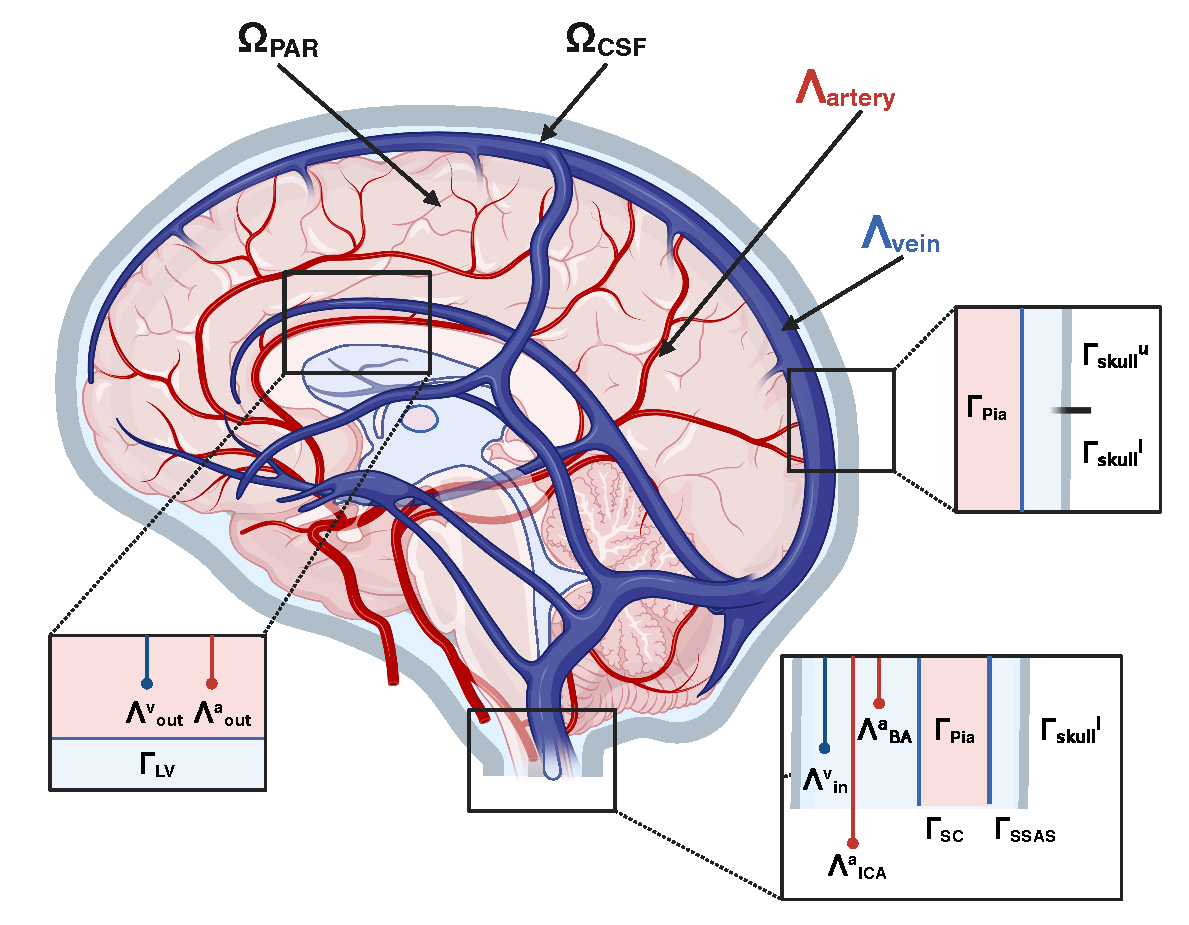
\includegraphics[width=\textwidth]{figures/Brain-PVS-callouts.pdf}
%%          \label{fig:intracranial_domains}
%%      \end{subfigure}
%%      \hfill
%%      \begin{subfigure}[b]{0.3\textwidth}
%%          \centering
%%          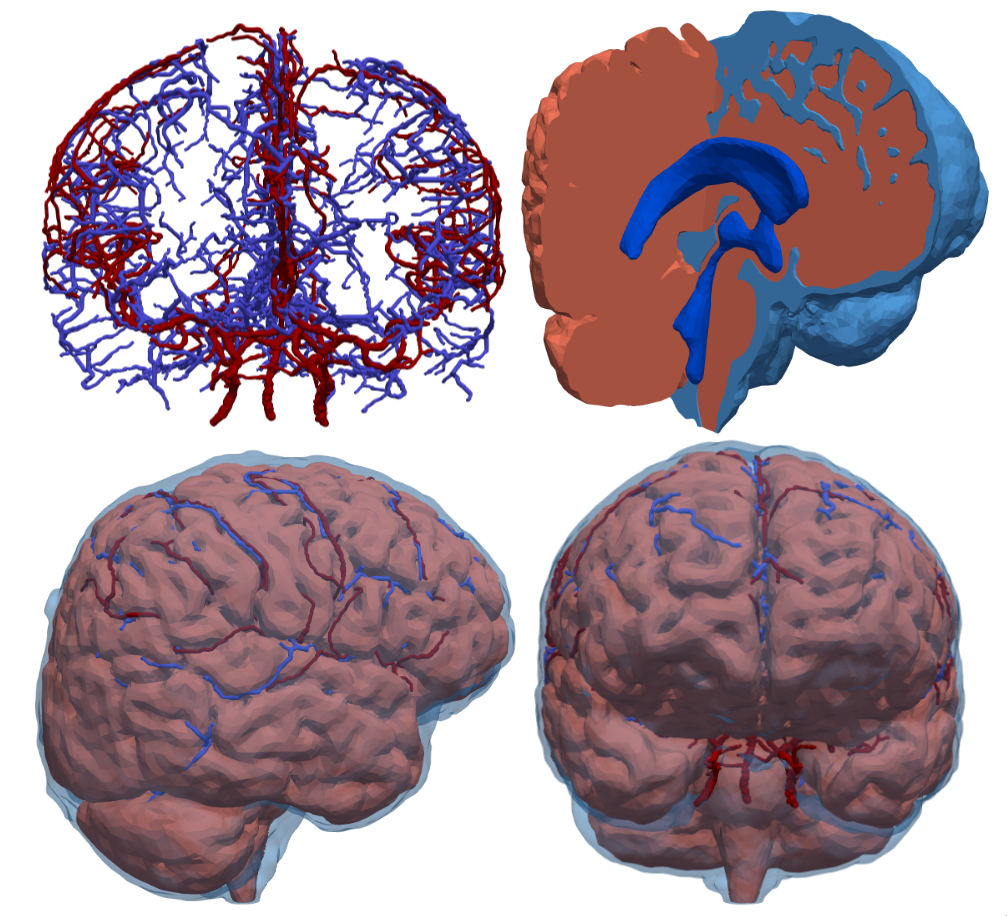
\includegraphics[width=\textwidth]{figures/geometry_concept.png}
%%          \caption{The arterial (red) and venous (blue) networks (top left), the parenchyma and CSF space (top right), combined (bottom row)}
%%          \label{fig:three sin x}
%%      \end{subfigure}
%%      \hfill
%%      \begin{subfigure}[b]{0.24\textwidth}
%%          \centering
%%          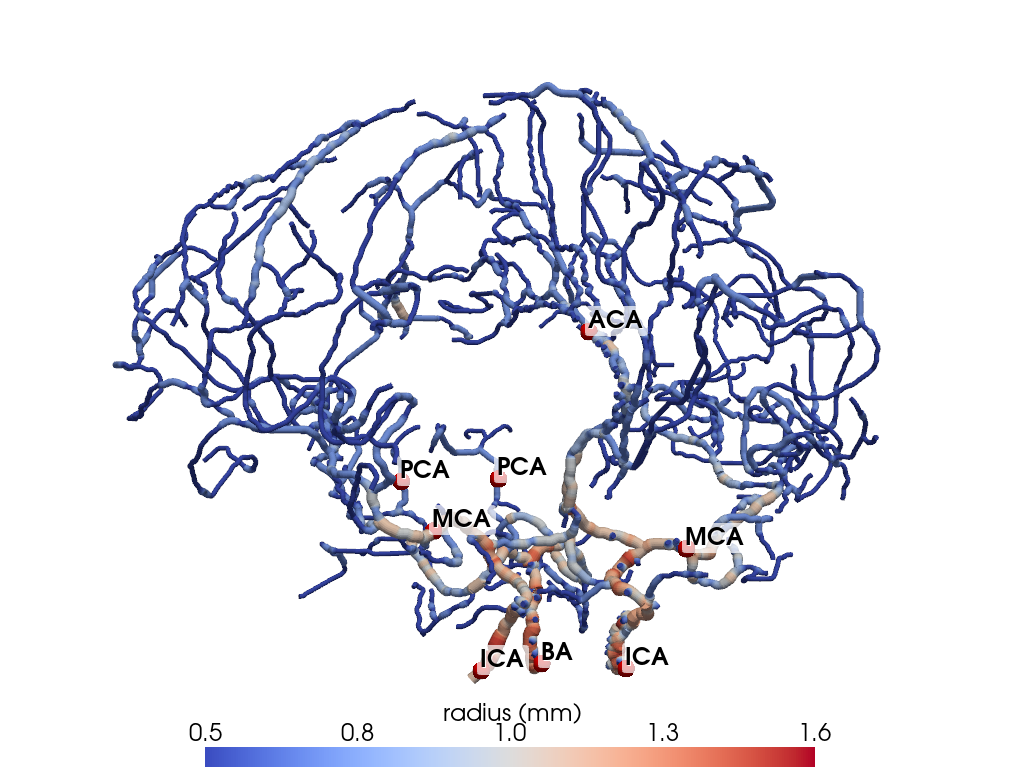
\includegraphics[trim={4cm 0 4cm 0},clip,width=\textwidth]{figures/labeled_arteries.png}
%%          \caption{The arterial network with the main cerebral arteries: internal carotid artery (ICA), middle cerebral artery (MCA), anterior cerebral artery (ACA) and posterior cerebral artery (PCA)}
%%          \label{fig:five over x}
%%      \end{subfigure}
%%      %\caption{@Marius: Starts adding parts of this. \mer{MER: Concept figure illustrating the compartments and story line. (A) Concept sketch of the SAS, PVS and the brain; (B) Visualization of geometry domains (brain, sas and vasculature; think about colors and associations; please don't make blood blue and water red e.g.) ; (C) Zoom-in/detail on vasculature, which are which arteries (ACA, MCA, PCA, CoW)  and veins (XXX); (D) Zoom-in 2 on vascular position versus SAS and brain; (E) Zoom-in 3 on where PVS ends; (F) Illustration of boundaries? (G) Concept illustration of the mathematical model (diffusion, convection, exchange, boundaries).}}
%% \label{fig:concept}
%% \end{figure}


\begin{table}
\begin{center}
  \begin{tabular}{ll|llllll|ll}
    \toprule
    & Description & $R$ & $\xi_{\rm PVS-SAS}$, $\xi_{\rm PVS-PAR}$ & $\beta_{\rm efflux}$ & $D$ & $\hat{u}$ & $\mathbf{u}_{\rm SAS, PAR}$ & $g_{\rm influx}$ & $c_0$ \\
    \midrule
    A & Baseline  & $R_2 = 2 R_1$ & $\xi$, $\tilde \xi$\cite{koch2023estimates} &  $10^{-4}$ mm$^2$/s\cite{hornkjol2022csf} & $D^{\rm gad}$\cite{sykova2008diffusion, valnes2020apparent}  & $\hat{u} = \hat{u}_{\rm prod}$ & $\mathbf{u}_{\rm SAS} = \mathbf{u}_{\rm prod}$, $\mathbf{u}_{\rm PAR} = 0$ & $> 0$ & 0 \\
    B & PVS "sheaths" & $R_2 = 2 R_1$ & $0, 0.5 \xi, \xi, 2 \xi, 1000 \xi \approx \infty$, --\cite{koch2023estimates} & -- & --  &  --  & --  & -- & -- \\
    C & Larger PVS & $R_2 = N R_1$ & -- & -- & --  &  --  & -- & -- & -- \\
    D & PVS I & $R_2 = 2 R_1$ & $\xi$, -- & -- & --  &  $\hat{u} = \hat{u}_{\rm prod} + \uparrow$  & -- & -- & -- \\
    E & PVS II & $R_2 = 2 R_1$ & $\xi$, -- & -- & --  &  $\hat{u} = \hat{u}_{\rm prod} + \uparrow\uparrow$  & -- & -- & -- \\
    F & PVS III & $R_2 = 2 R_1$ & $\xi$, -- & -- & $10 D_{\rm PVS}$ &  $\hat{u} = \hat{u}_{\rm prod}$  & -- & -- & -- \\
    G & Glymphatics & $R_2 = 2 R_1$ & $\xi$, -- & -- & \cite{sykova2008diffusion, valnes2020apparent} &  $\hat{u} = \hat{u}_{\rm prod} + \uparrow$  & $\mathbf{u}_{\rm PAR}$ > 0 & -- & -- \\
    H & Sleep &  &  & &  &  &  & & \\
    I & Pathology I &  &  & &  &  &  & & \\
    J & Pathology II &  &  & &  &  &  & & \\
    \midrule
    X & Clearance & $R_2 = 2 R_1$ & $50\%$, $\xi$ & -- & $D^{\rm gad, \tau, A\beta}$  &  $\hat{u} = \hat{u}_{\rm prod}$  & -- & $0$ & $1$ \\
    Y & (PVS) & $R_2 = 2 R_1$ & $50\%$, $\xi$ & -- & $D^{\rm gad, \tau, A\beta}$  &  $\hat{u} = \hat{u}_{\rm prod} + \uparrow$  & -- & -- & -- \\
    Z & (Glymphatic) & $R_2 = 2 R_1$ & $50\%$, $\xi$ & -- & $D^{\rm gad, \tau, A\beta}$  &  $\hat{u} = \hat{u}_{\rm prod} + \uparrow$  & $\mathbf{u}_{\rm PAR}$ > 0 & -- & -- \\
    \bottomrule
    \end{tabular}
    \end{center}
\caption{Overview of models (-- denotes as immediately above). Model A represents a baseline scenario with semi-permeable barriers between the PVS and SAS ($\xi_{\rm PVS-SAS} \approx 50\%$, \mer{we try to estimate this value by a bit of trial-and-error from the observations of timings of PVS-SAS and SAS from~\cite{eide2024functional}})~\cite{bedussi2017paravascular} and astrocytic endfeet forming barriers within the parenchyma~\cite{koch2023estimates}. $R_1$ and $R_2$ denotes the inner and outer radius of the PVS, with PVS width comparable to vascular diameter ($R_2 - R_1 \approx 2 R_1$)\cite{mestre2018flow} as a baseline. The extracranial solute efflux permeability $\beta_{\rm efflux}$ is uniformly distributed over the outer SAS boundary with a reasonable rate as baseline\cite{hornkjol2022csf, eide2021clinical, ringstad2024glymphatic}. At baseline, the effective diffusion coefficients $D^{\rm x}_{\rm SAS} = D^{\rm x}_{\rm PVS}$ of the SAS and PVS represent the free diffusion coefficient of Gadubutrol (${\rm x} = {\rm gad}$) in CSF (water), and $D^{\rm x}_{\rm PAR}$ the effective diffusion coefficient of human cortical tissue, all at body temperature. At baseline, we consider net flow due to CSF-production in the SAS (and PVS): $\mathbf{u}_{\rm SAS} > 0$ (and $\hat{u} > 0$), but no additional effects from perivascular pulsatility nor bulk flow in the parenchyma $\mathbf{u}_{\rm PAR} = 0$. Due to the timescale for human intracranial tracer transport (minutes to hours) compared to typical (cardiac, respiratory, slow vasomotion) human intracranial pulsatility (0.1 -- 1 Hz), we consider net (constant-in-time) flow fields only in subsequent model variations. Model B represents a PVS-SAS interface configuration with minimal or more permeable structural barriers~\cite{eide2024functional}, while Model C represents enlarged PVS. Models D, E, and F represent three perivascular pathway scenarios with more rapid flow in the PVS induced by vasomotion (PVS I)~\cite{gjerde2023directional} or a net fluid source in the PVS (1D Stokes flow)/net pressure difference between PVS inlets and outlets (PVS II), or with enhanced effective diffusion due to mixing (PVS III)~\cite{hornkjol2022csf, troyetsky2021dispersion, vinje2023human}, respectively. Model G attempts to represent a glymphatic--like convective flow within the parenchyma. \mer{Ideas could be:  (a) network induces arterial and venous sources in a Darcy porous media flow model (reflects the glymphatic hypothesis), (b) Croci-style \cite{croci2019uncertainty}, (c) \cite{vinje2023human}} Model H represents physiological alterations associated with sleep (lower CSF production, enhanced diffusion within the parenchyma, enhanced PVS pulsatility), while Models I--J represents variations associated with pathologies (e.g.~dementia, hypertension, angiopathies, CSF-disorders and/or others). Models X--Z represent version of the aforementioned scenarios but for studying metabolite clearance (instead of solute influx).}
\label{tab:scenarios}
\end{table}
